\documentclass{beamer}
\usepackage[utf8]{inputenc}

\usetheme{Madrid}
\usecolortheme{default}
\usepackage{amsmath,amssymb,amsfonts,amsthm}
\usepackage{txfonts}
\usepackage{multicol}
\usepackage{tkz-euclide}
\usepackage{listings}
\usepackage{adjustbox}
\usepackage{array}
\usepackage{tabularx}
\usepackage{gvv}
\usepackage{lmodern}
\usepackage{circuitikz}
\usepackage{tikz}
\usepackage{graphicx}
\usepackage{hyperref}
\usepackage{siunitx}

\setbeamertemplate{page number in head/foot}[totalframenumber]

\usepackage{tcolorbox}
\tcbuselibrary{minted,breakable,xparse,skins}



\definecolor{bg}{gray}{0.95}
\DeclareTCBListing{mintedbox}{O{}m!O{}}{%
  breakable=true,
  listing engine=minted,
  listing only,
  minted language=#2,
  minted style=default,
  minted options={%
    linenos,
    gobble=0,
    breaklines=true,
    breakafter=,,
    fontsize=\small,
    numbersep=8pt,
    #1},
  boxsep=0pt,
  left skip=0pt,
  right skip=0pt,
  left=25pt,
  right=0pt,
  top=3pt,
  bottom=3pt,
  arc=5pt,
  leftrule=0pt,
  rightrule=0pt,
  bottomrule=2pt,
  toprule=2pt,
  colback=bg,
  colframe=orange!70,
  enhanced,
  overlay={%
    \begin{tcbclipinterior}
    \fill[orange!20!white] (frame.south west) rectangle ([xshift=20pt]frame.north west);
    \end{tcbclipinterior}},
  #3,
}
\lstset{
    language=C,
    basicstyle=\ttfamily\small,
    keywordstyle=\color{blue},
    stringstyle=\color{orange},
    commentstyle=\color{green!60!black},
    numbers=left,
    numberstyle=\tiny\color{gray},
    breaklines=true,
    showstringspaces=false,
}
%------------------------------------------------------------
%This block of code defines the information to appear in the
%Title page
\title %optional
{12.18}
\date{October 5,2025}
%\subtitle{A short story}

\author % (optional)
{Aditya Appana - EE25BTECH11004}



\begin{document}


\frame{\titlepage}
\begin{frame}{Question}
$\vec{X}$ is 1 km northeast of $\vec{Y}$. $\vec{Y}$ is 1 km southeast of $\vec{Z}$. $\vec{W}$ is 1 km west of $\vec{Z}$. $\vec{P}$ is 1
km south of $\vec{W}$. $\vec{Q}$ is 1 km east of $\vec{P}$. What is the distance between $\vec{X}$ and $\vec{Q}$ in km?
\begin{enumerate}
\begin{multicols}{4}
    \item 1
    \item $\sqrt{2}$
    \item $\sqrt{3}$
    \item 2
\end{multicols}
\end{enumerate}
\end{frame}



\begin{frame}[fragile]
    \frametitle{Solution}
Let $\vec{X}$ be $\myvec{0\\0}$. Every subsequent vector can be expressed as a translation by a unit vector, from the previous vector. The translation vector can be represented as:\\
\begin{align}
\myvec{\cos\theta \\ \sin\theta}
\end{align}
\end{frame}


\begin{frame}[fragile]
    \frametitle{Solution}
$\vec{X}$ is 1km north-east of $\vec{Y}$, so $\vec{Y}$ is 1km south-west of $\vec{X}$. Therefore:\begin{align}
\vec{Y}-\vec{X} = \myvec{\cos225\degree \\ \sin225\degree}\\
\vec{Y}-\vec{X} = \myvec{\frac{-1}{\sqrt{2}}\\\frac{-1}{\sqrt{2}}}
\end{align}\\
$\vec{Y}$ is 1km south-east of $\vec{Z}$, so $\vec{Z}$ is 1km north-west of $\vec{Y}$. Therefore:\begin{align}
\vec{Z}-\vec{Y} = \myvec{\cos135\degree \\ \sin135\degree}\\
\vec{Z}-\vec{Y} = \myvec{\frac{-1}{\sqrt{2}}\\\frac{1}{\sqrt{2}}}
\end{align}\\
\end{frame}

\begin{frame}[fragile]
    \frametitle{Solution}
$\vec{W}$ is 1km west of $\vec{Z}$. Therefore:\begin{align}
\vec{W}-\vec{Z} = \myvec{\cos180\degree \\ \sin180\degree}\\
\vec{W}-\vec{Z} = \myvec{-1\\0}
\end{align}\\
$\vec{P}$ is 1km south of $\vec{W}$. Therefore:\begin{align}
\vec{P}-\vec{W} = \myvec{\cos270\degree \\  \cos270\degree}\\
\vec{P}-\vec{W} = \myvec{0\\-1}
\end{align}\\
\end{frame}

\begin{frame}[fragile]
    \frametitle{Solution}
$\vec{Q}$ is 1km east of $\vec{P}$. Therefore:\begin{align}
\vec{Q}-\vec{P} = \myvec{\cos0\degree \\ \sin0\degree}\\
\vec{Q}-\vec{P} = \myvec{1\\0}
\end{align}\\
Adding (3), (5), (7), (9), (11) together, we get $\vec{Q}-\vec{X} =\vec{Q} = \myvec{-\sqrt{2}\\-1}$.
\end{frame}

\begin{frame}[fragile]
    \frametitle{Solution}
The distance between $\vec{X}=\myvec{0\\0}$ and $\vec{Q}=\myvec{-\sqrt{2}\\-1}$ is:
\begin{align}
    ||\vec{X} - \vec{Q}||= \norm{\myvec{\sqrt{2}\\1}} \\
    \sqrt{(\sqrt{2})^2 +1^2} = \sqrt{3}
\end{align}\\
Therefore the correct option is \textbf{C}.
\end{frame}

\begin{frame}[fragile]
    \frametitle{Code}
\href{https://github.com/AdityaAppana/ee1030-2025/tree/96431e23cc4d088e70368e400c3c60fbecfcaaa8/ee25btech11004/matgeo/12.18/Codes}{Codes Permalink}
\end{frame}

\begin{frame}[fragile]
    \frametitle{Figure}
\begin{figure}[H]
    \centering
    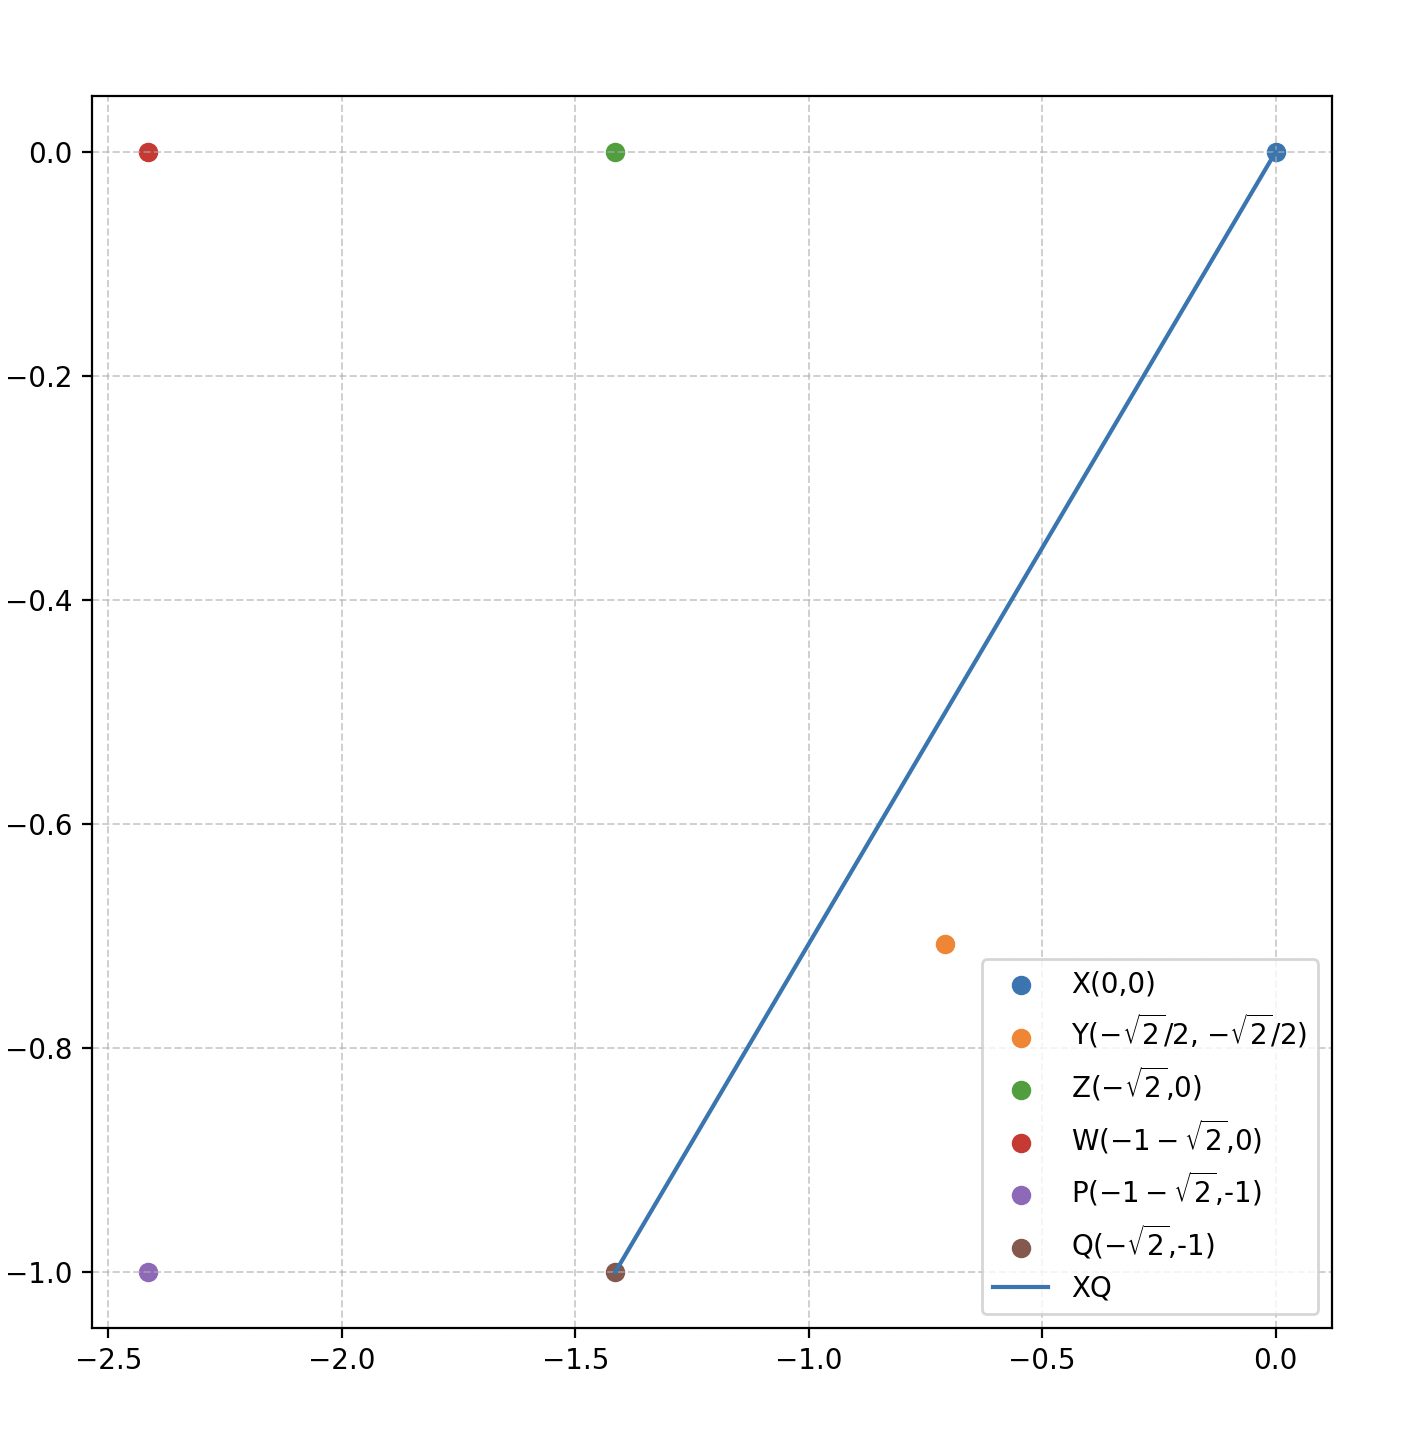
\includegraphics[width=0.6\columnwidth]{Figs/1218.png}
    \caption{Plot}
    \label{fig:placeholder}
\end{figure}
\end{frame}

\end{document}